\documentclass[tikz, border=0pt]{standalone}
\usepackage{tikz}

\newcommand\startx{0}
\newcommand{\norm}[1]{\left\lVert#1\right\rVert}

\begin{document}
	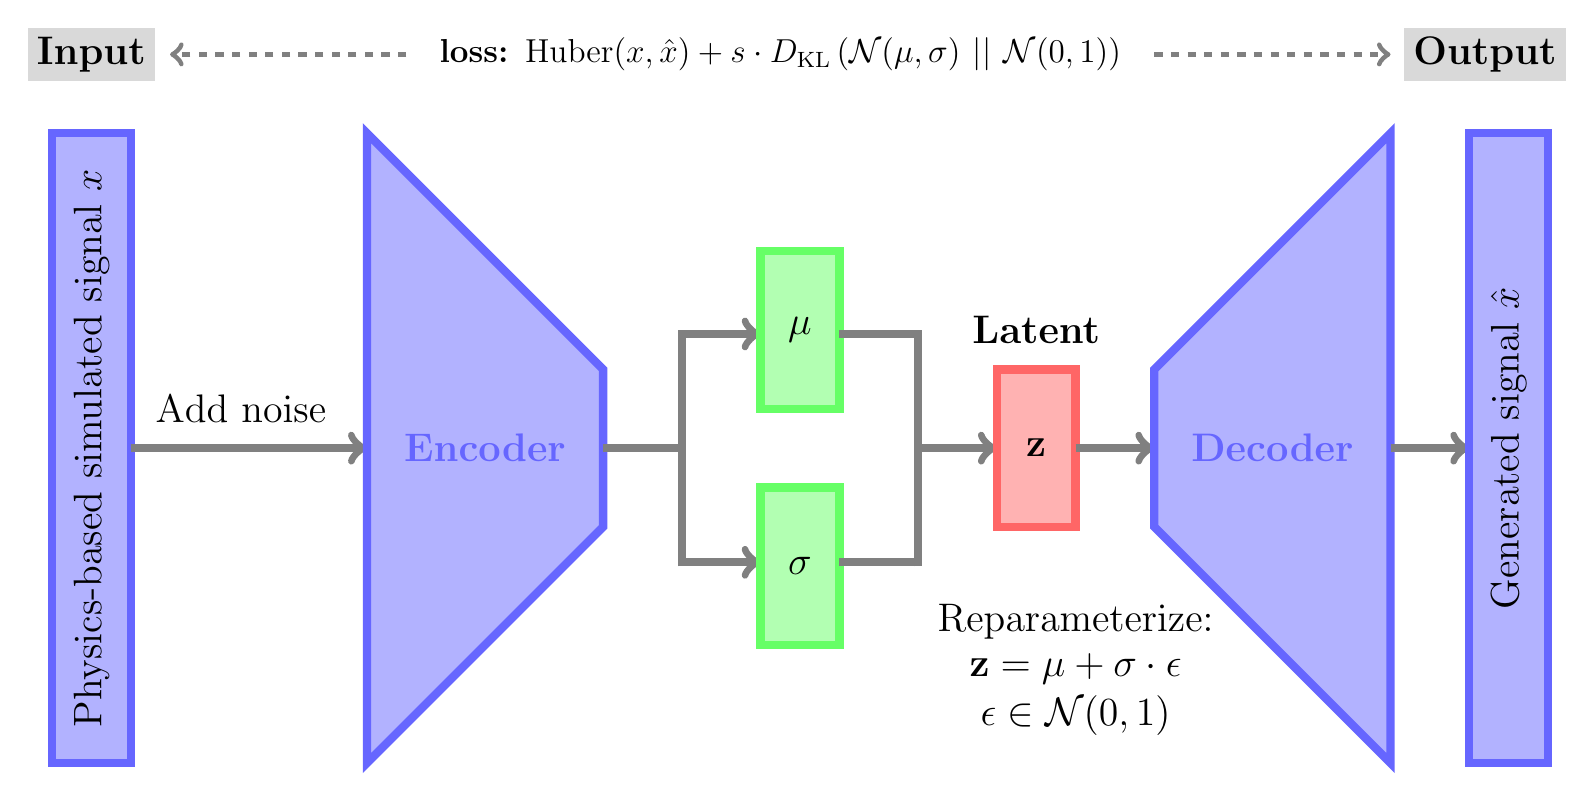
\begin{tikzpicture}
		\draw[fill=blue!30, draw=blue!60, line width=3pt] (\startx, 0) rectangle (\startx+1, 8);
		\node[font=\Large, rotate=90] at (\startx+0.5,4) {Physics-based simulated signal $x$};

        \node[font=\Large] at (\startx+2.4, \startx+4.5) {Add noise};
		\draw[->, gray, thick, line width=3pt] (\startx+1, 4) -- (\startx+4, 4);

		\draw[fill=blue!30, draw=blue!60, line width=3pt] (4,8) -- (4,0) -- (7,3) -- (7,5) -- cycle;
		\node[text=blue!60, font=\Large] at (5.5,4) {\textbf{Encoder}};

		\draw[- , gray, thick, line width=3pt] (7,4) -- (8,4);
		\draw[- , gray, thick, line width=3pt] (8,2.5) -- (8,5.5);
		\draw[->, gray, thick, line width=3pt] (8,5.45) -- (9,5.45);  % to mu
		\draw[->, gray, thick, line width=3pt] (8,2.55) -- (9,2.55);  % to sigma

		\draw[fill=green!30, draw=green!60, line width=3pt] (9, 4.5) rectangle (10, 6.5);
		\node[font=\Large] at (9.5, 5.5) {$\mathbf{\mu}$};

		\draw[fill=green!30, draw=green!60, line width=3pt] (9, 1.5) rectangle (10, 3.5);
		\node[font=\Large] at (9.5, 2.5) {$\mathbf{\sigma}$};

		\draw[- , gray, thick, line width=3pt] (10,5.45) -- (11,5.45);
		\draw[- , gray, thick, line width=3pt] (10,2.55) -- (11,2.55);
		\draw[- , gray, thick, line width=3pt] (11,2.5) -- (11,5.5);  % to mu
		\draw[->, gray, thick, line width=3pt] (11,4) -- (12,4);  % to sigma


		\draw[fill=red!30, draw=red!60, line width=3pt] (12, 3) rectangle (13, 5);
		\node[font=\Large] at (12.5, 4) {$\mathbf{z}$};
		\node[font=\Large] at (12.5, 5.5) {\textbf{Latent}};

        \node[font=\Large] at (13, 1.8) {Reparameterize:};
		\node[font=\Large] at (13, 1.2) {$\mathbf{z} = \mathbf{\mu} + \mathbf{\sigma} \cdot \mathbf{\epsilon}$};
		\node[font=\Large] at (13, 0.6) {$\mathbf{\epsilon} \in \mathcal{N} (0, 1)$};

		\draw[->, gray, thick, line width=3pt] (13, 4) -- (14, 4);

		\draw[fill=blue!30, draw=blue!60, line width=3pt] (14,3) -- (14,5) -- (17,8) -- (17,0) -- cycle;
		\node[text=blue!60, font=\Large] at (15.5,4) {\textbf{Decoder}};

		\draw[->, gray, thick, line width=3pt] (17, 4) -- (18, 4);

		\draw[fill=blue!30, draw=blue!60, line width=3pt] (18, 0) rectangle (19, 8);
		\node[font=\Large, rotate=90] at (18.5,4) {Generated signal $\hat{x}$};


		\node[text=black, font=\Large, fill=gray!30] at (0.5,9) {\textbf{Input}};
		\node[text=black, font=\Large, fill=gray!30] at (18.2,9) {\textbf{Output}};

		\draw[->, gray, thick, dashed, line width=2pt] (4.5, 9) -- (1.5, 9);
		\draw[->, gray, thick, dashed, line width=2pt] (14, 9) -- (17.0, 9);

		\node[text=black, font=\large] at (9.25,9) {\textbf{loss: $\mathrm{Huber}(x, \hat{x}) + s \cdot D_\mathrm{KL}\left( \mathcal{N}(\mu, \sigma)~||~\mathcal{N}(0, 1) \right)$}};
	\end{tikzpicture}
\end{document}
